
% Our goal is to merge any models of the same architecture together \textit{without additional training}. Unlike prior work \cite{wortsman2022model,ainsworth2022git,jordan2022repair}, we specifically target the extremely difficult setting of models that have different initializations and are trained on completely different tasks. In this section, we will motivate the need for a new approach by showing how prior work fails on this challenging setting.

% \paragraph{What constitutes a task?}
% The term ``task'' is often overloaded in machine learning. The broader vision community treats ``tasks'' as different problem statements (e.g., detection vs. segmentation \cite{lin2014coco}), while subfields like continual learning \cite{de2021continual} define ``tasks'' as disjoint category splits of the same data. While we would ideally support any definition, we specifically focus on classification in this work. We define tasks as either disjoint category splits of the same data or as classification on different datasets entirely.

% \subsection{Background}
% Consider a model $\mathcal{L}$ as a collection of layers $L_i \in \mathcal{L}$, each of which may have some parameters (e.g., $W_i, b_i$ for a linear layer). 
% If \modela{$\mathcal{L}^A$} and \modelb{$\mathcal{L}^B$} are finetuned from the same checkpoint, several works (e.g., \cite{huang2017snapshot,izmailov2018averaging,wortsman2022model}) have found that merging them is as easy as averaging their weights. For instance, if $L_i$ is a linear layer, the new weight matrix \modelc{$W_i^*$} is simply
% \begin{equation} \label{eq:wavg}
%     % \modelc{W_i^*} = \modela{\frac{1}{2} W_i^A} + \modelb{\frac{1}{2} W_i^B}
%     \modelc{W_i^*} = \gamma\modela{W_i^A} + (1-\gamma)\modelb{W_i^B}
% \end{equation}
% \textcolor{blue}{where $\gamma\in[0,1]$ and is usually set to $\frac{1}{2}$.} 
% However, if \modela{$\mathcal{L}^A$} and \modelc{$\mathcal{L}^B$} were not finetuned from the same checkpoint, Eq.~\ref{eq:wavg} typically results in random accuracy
% To fix this, a line of work (most recently \cite{ainsworth2022git,jordan2022repair}) has found that if you first permute the feature space of one model to align with the feature space of the other model before averaging them together, you can recover much of the lost accuracy. More concretely, let \modelb{$P_i$} be a permutation matrix that permutes the output of layer \modelb{$L_i^B$} to the space of \modela{$L_i^A$}. Then for each layer, works such as Git Re-Basin \cite{ainsworth2022git} apply
% \begin{equation} \label{eq:rebasin}
%     % \modelc{W_i^*} = \modela{\frac{1}{2} W_i^A} + \modelb{\frac{1}{2} P_i W_i^B P_{i-1}^T}
%     \modelc{W_i^*} = \gamma\modela{W_i^A} + (1-\gamma)\modelb{ P_i W_i^B P_{i-1}^T}
% \end{equation}
% Note that here we permute the output space of \modelb{$W_i^B$}, but we also need to permute its input space to undo the permutation from the previous layer (hence the use of \modelb{$P_{i-1}^T$}).

% 
% \begin{wrapfigure}{r}{0.48\textwidth}
%   \vspace{-20pt}
%   \centering
%   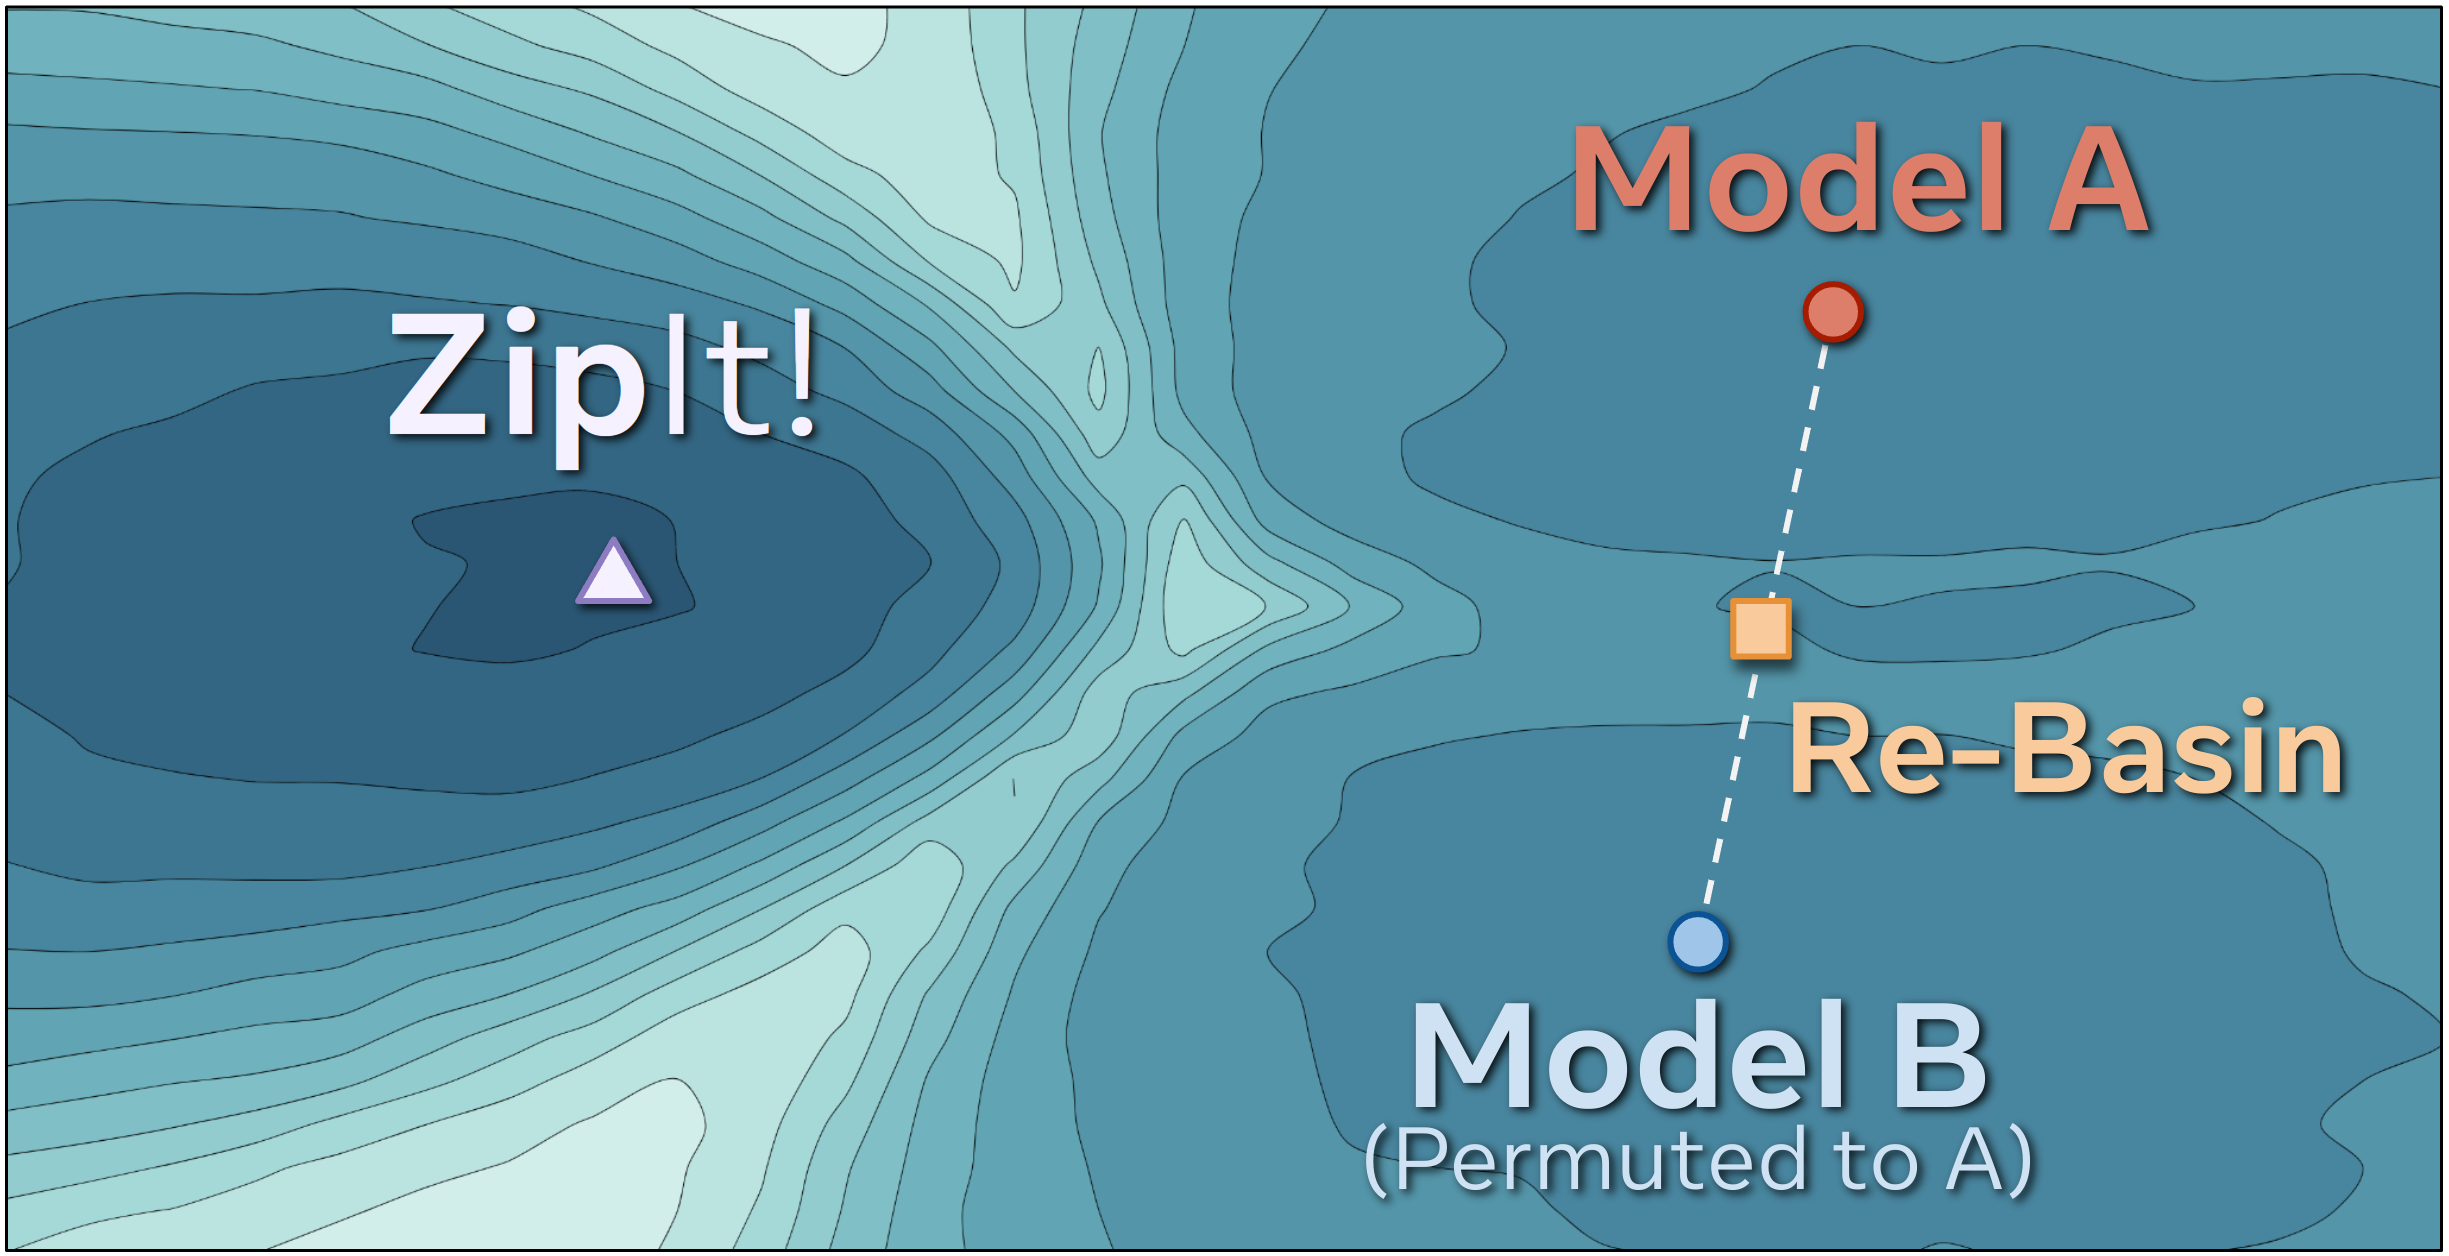
\includegraphics[width=\linewidth]{figures/imgs/loss_basin.png}
%   \newline
%   \caption{{\bf Prior Work Fails} on merging models trained on \textit{different} tasks. Git Re-Basin \cite{ainsworth2022git} assumes the two models lie in the same loss basin \textit{modulo permutation} and interpolates between them. However, that is not sufficient when the models are trained on \textit{different} tasks, here shown for disjoint class sets of CIFAR-100. While \modela{A} and the permuted \modelb{B} lie in similar basins, Git Re-Basin's interpolation performs \textit{worse} than the originals. In contrast, our method \name\ merges them into an even better model in a completely different loss basin.}
%   \label{fig:loss_basin}
%   \vspace{-50pt}
% \end{wrapfigure}



\begin{figure}
  \centering
  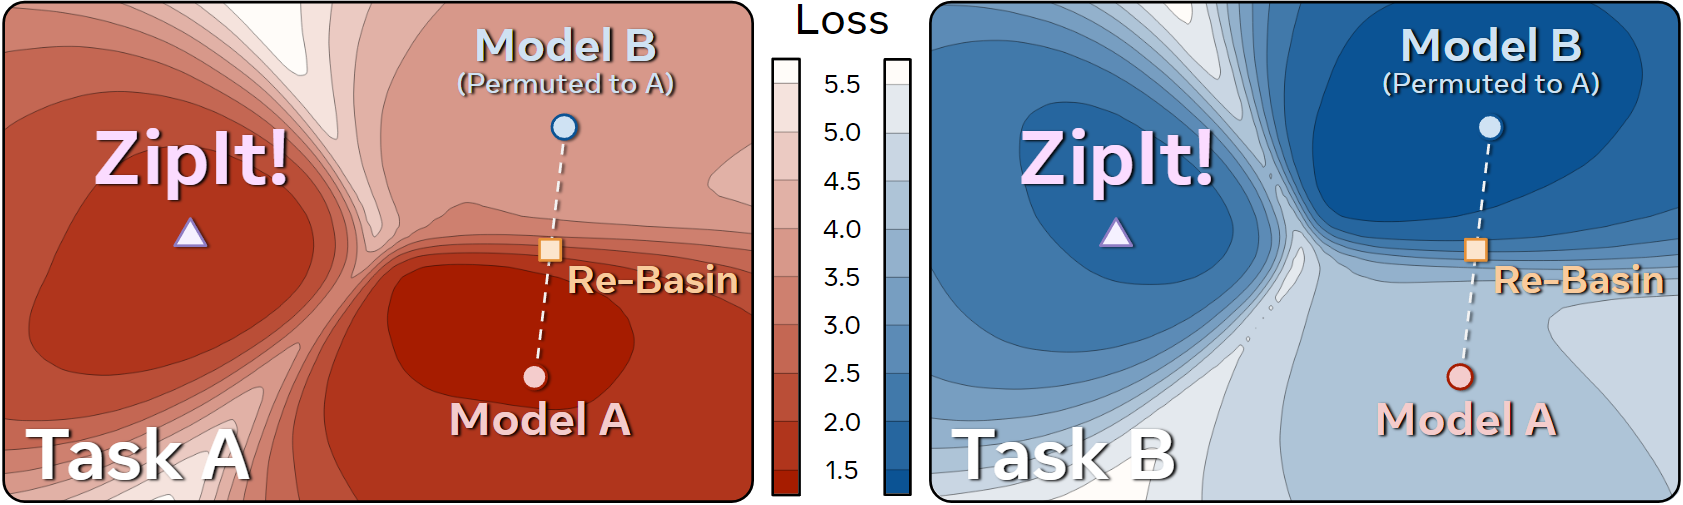
\includegraphics[width=\linewidth]{figures/imgs/loss_landscapes.png}
  % \newline
  % \vspace{-0.5em}
  \caption{{\bf Task Loss Landscapes} for models in Tab.~\ref{tab:cifar50+50}. % Prior work fails on merging models trained on different tasks: 
  \modela{Model A} and \modelb{Model B} lie in low loss basins for their own tasks, but \textit{not for the other task}.
  % While \modelb{Model B} lies in a low loss basin for \modelb{Task B}, it doesn't for \modela{Task A}, even after permuting it to \modela{Model A}.
  % because permuted models for \modela{Task A} likely \textit{do not} lie in a low loss basin for \modelb{Task B}.
  Thus, any interpolation between \modela{Model A} and a permuted \modelb{Model B} (e.g., Git Re-basin) lies outside the minima \textit{for both tasks} and thus performs poorly. In contrast, \name{}\ improves the merge by finding a model that lies in a low loss basin for both.
  % by finding a loss basin common to both tasks.
  % Git Re-Basin~\citet{ainsworth2022git} assumes the two models likely lie in the same loss basin \textit{modulo permutation} and interpolates between them. However, this is substantially less likely when the models are trained on \textit{different} tasks, here shown for disjoint class sets of CIFAR-100. While \modela{A} and \modelb{B} lie in basins on their respective tasks, these \textit{are not} shared across tasks. Thus, Git Re-Basin's interpolation performs \textit{worse} than the original's. In contrast, our method \name{}\ significantly improves the merge by finding a basin common to both tasks. 
  }
  \label{fig:loss_basin}
\end{figure}
% \paragraph{Problems with Permutation.}
% While Eq.~\ref{eq:rebasin} works decently well for models trained on the same task, its underlying assumptions break down when the models are trained on \textit{different} tasks. The idea of permutation-based model merging (e.g. Git Re-Basin \cite{ainsworth2022git}) stems from mode connectivity \cite{entezari2021role}, where it has been conjectured that models with different initializations trained on the same data lie in the same \textit{loss basin} (i.e., region of low loss or high accuracy) modulo permutation (as most neural networks can be permuted internally without affecting their outputs). As we show in Fig.~\ref{fig:loss_basin}, this does not hold in our setting where the two models are trained on different tasks. In this case, \modelb{Model B}'s optimal permutation lies in a \textit{similar} yet distinct basin to \modela{Model A}. Because the two models are actually in \textit{different basins}, the interpolated result actually has a \textit{lower} accuracy than either of the two original models. This motivates us to explore alternative methods for merging.

\section{Background and Motivation} \label{sec:motivation}

%%%%%%%%%%%%%%%%%%%%%%%%%%%%%%%%%%% NEW EDITS %%%%%%%%%%%%%%%%%%%%%%%%%%%%%%%%%%%
% The idea of 
Model merging stems from mode connectivity \cite{garipov2018loss}, where it is conjectured that models trained with SGD on the same dataset lying in the same \textit{loss basin} (i.e., region or \textit{mode} of low loss) can be combined into a single model that's just as performant as the original models. If these models can be combined well by linearly interpolating their weights, they are said to be \textit{linearly mode connected} (LMC) \cite{garipov2018loss,entezari2021role}. Our work is similar to finding LMC, but across \textit{different datasets with disjoint label sets} (i.e., separate tasks as in \citet{de2021continual}).

Consider a model $\mathcal{L}$ as a collection of layers $L_i \in \mathcal{L}$, each of which may have some parameters (e.g., $W_i, b_i$ for a linear layer). 
If \modela{$\mathcal{L}^A$} and \modelb{$\mathcal{L}^B$} are finetuned from the same checkpoint, several works (e.g., \citet{izmailov2018averaging,wortsman2022model}) find merging them is as easy as linearly interpolating their weights (i.e., they are LMC). E.g., if $L_i$ is a linear layer, the new weight matrix \modelc{$W_i^*$} is simply
\begin{equation} \label{eq:wavg}
    \modelc{W_i^*} = \gamma\modela{W_i^A} + (1-\gamma)\modelb{W_i^B}
\end{equation}
with an interpolation constant $\gamma\in[0,1]$, usually set to $\sfrac{1}{2}$. However, if \modela{$\mathcal{L}^A$} and \modelc{$\mathcal{L}^B$} were not finetuned from the same checkpoint, they often do not lie in the same mode \cite{entezari2021role, ainsworth2022git} and cannot be interpolated. Indeed, Eq.~\ref{eq:wavg} typically results in random accuracy. 

To fix this, \citet{entezari2021role} conjecture that \textit{large enough} models are likely LMC modulo permutation. This is because (1) many neural networks can be permuted internally without affecting their outputs and (2) permutation can move two models into the same basin, allowing much of the lost accuracy to be recovered.
% This is because permutations can move two models into the same basin without affecting their outputs, allowing much of the lost accuracy to be recovered.
More concretely, let \modelb{$P_i$} be a permutation matrix that permutes outputs of layer \modelb{$L_i^B$} to the space of \modela{$L_i^A$}. Then for each layer, permutation works 
% such as Git Re-Basin \cite{ainsworth2022git} 
apply
\begin{equation} \label{eq:rebasin}
    % \modelc{W_i^*} = \modela{\frac{1}{2} W_i^A} + \modelb{\frac{1}{2} P_i W_i^B P_{i-1}^T}
    \modelc{W_i^*} = \gamma\modela{W_i^A} + (1-\gamma)\modelb{ P_i W_i^B P_{i-1}^T}
\end{equation}
Note that here we permute the output space of \modelb{$W_i^B$}, but we also need to permute its input space to undo the permutation from the previous layer (hence the use of \modelb{$P_{i-1}^T$}).


% \begin{wrapfigure}{r}{0.48\textwidth}
%   \vspace{-20pt}
%   \centering
%   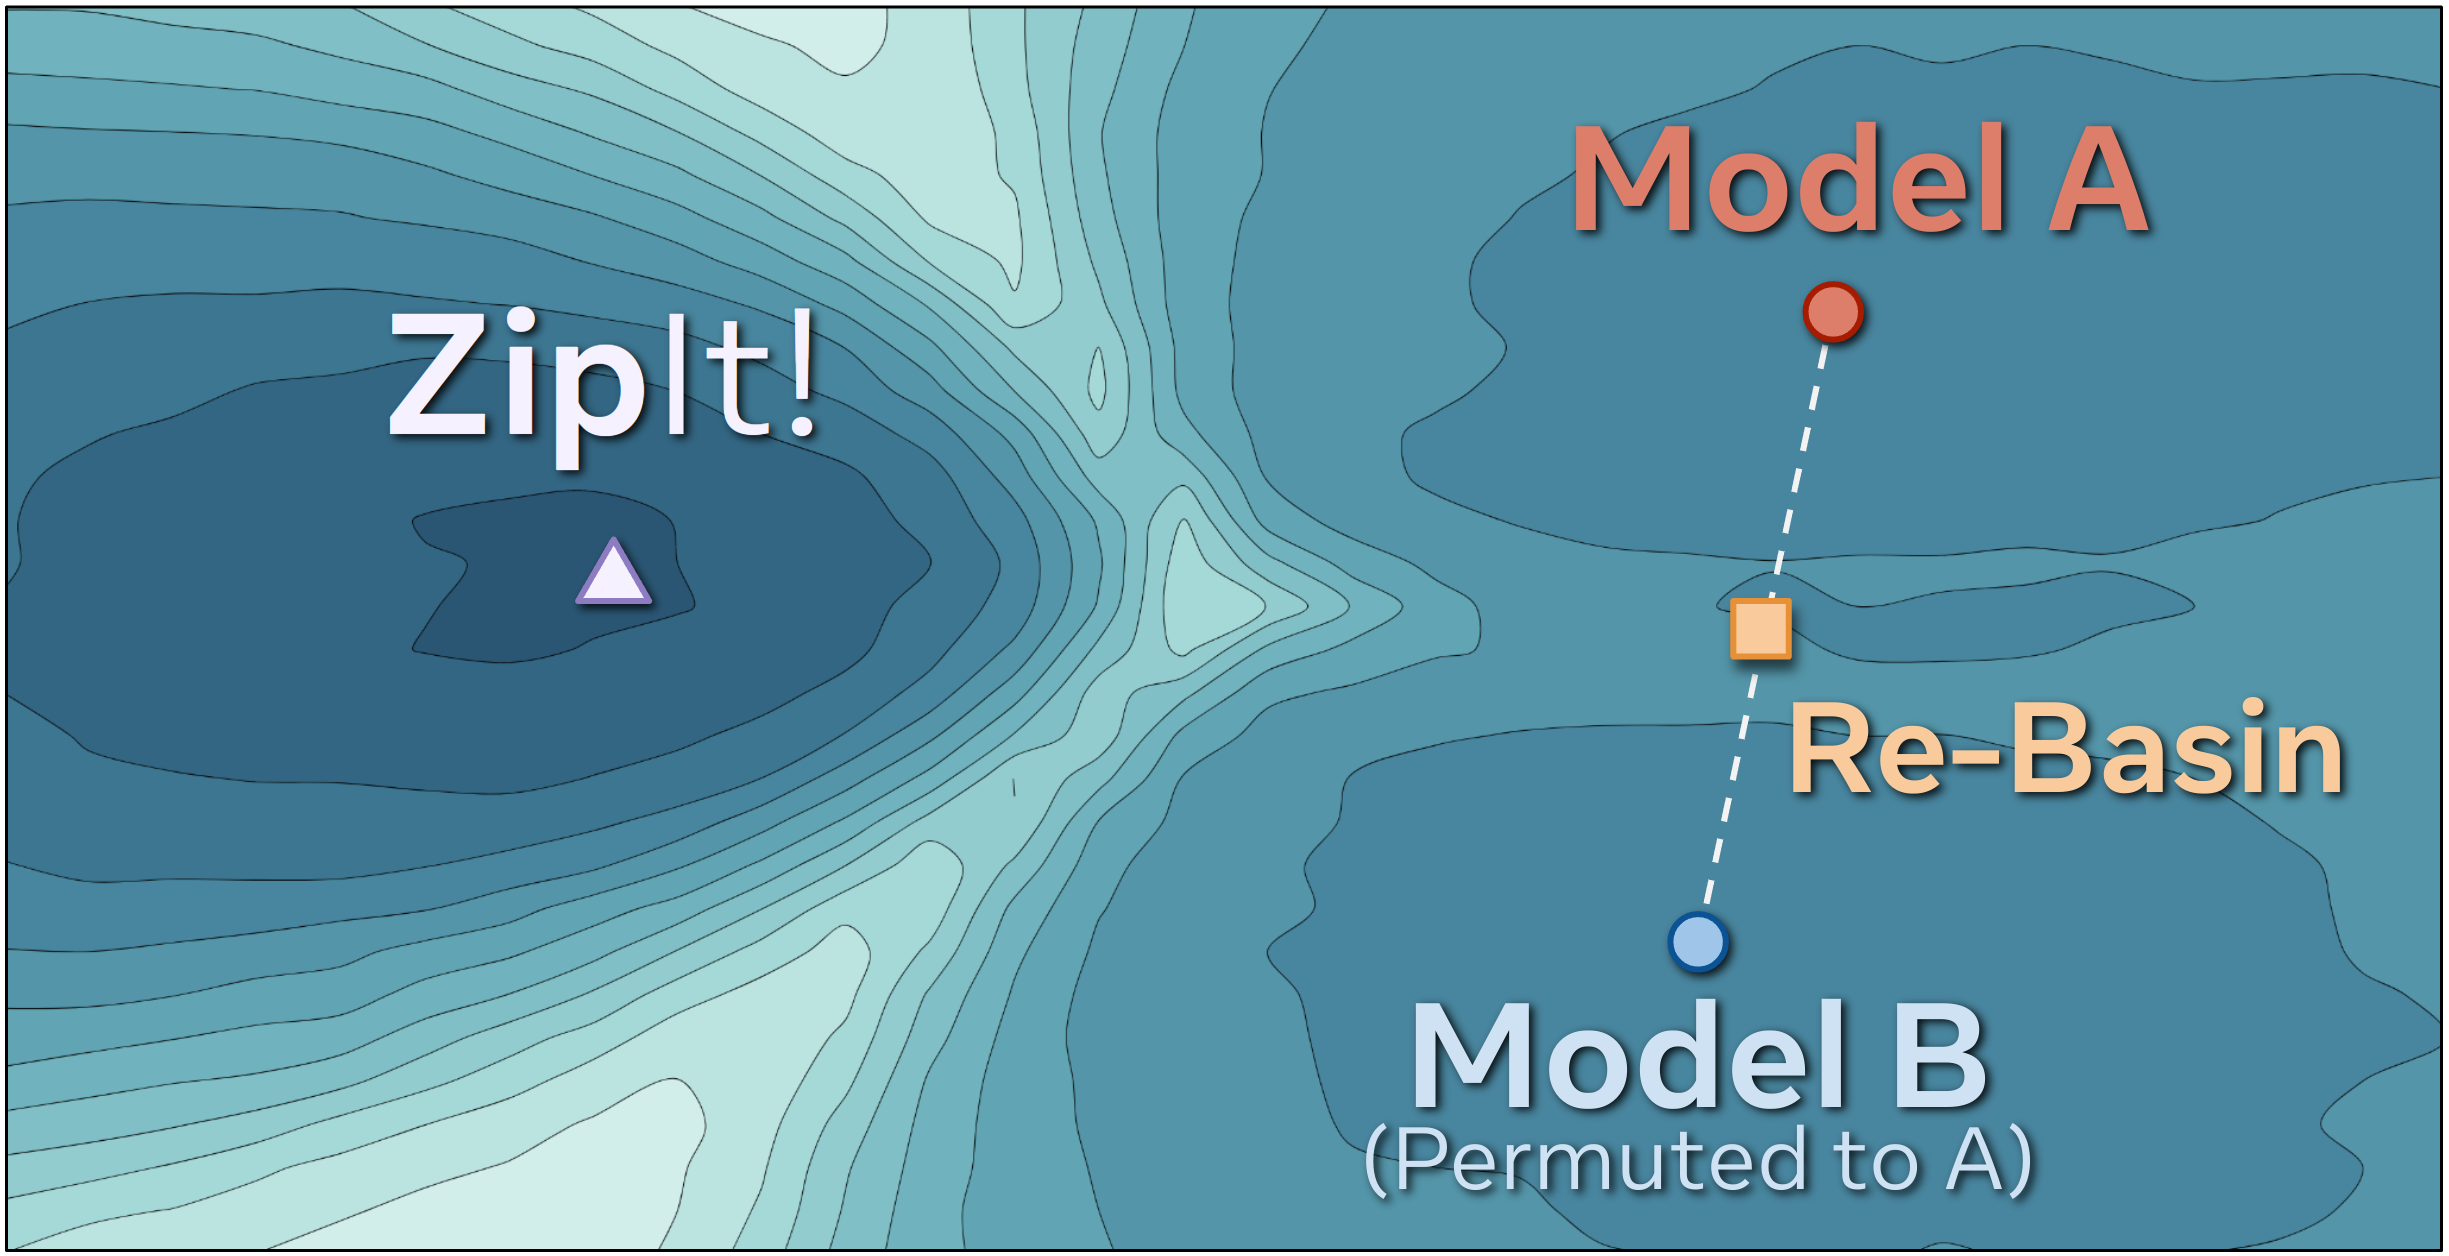
\includegraphics[width=\linewidth]{figures/imgs/loss_basin.png}
%   \newline
%   \caption{{\bf Prior Work Fails} on merging models trained on \textit{different} tasks. Git Re-Basin \cite{ainsworth2022git} assumes the two models lie in the same loss basin \textit{modulo permutation} and interpolates between them. However, that is not sufficient when the models are trained on \textit{different} tasks, here shown for disjoint class sets of CIFAR-100. While \modela{A} and the permuted \modelb{B} lie in similar basins, Git Re-Basin's interpolation performs \textit{worse} than the originals. In contrast, our method \name\ merges them into an even better model in a completely different loss basin.}
%   \label{fig:loss_basin}
%   \vspace{-50pt}
% \end{wrapfigure}



\begin{figure}
  \centering
  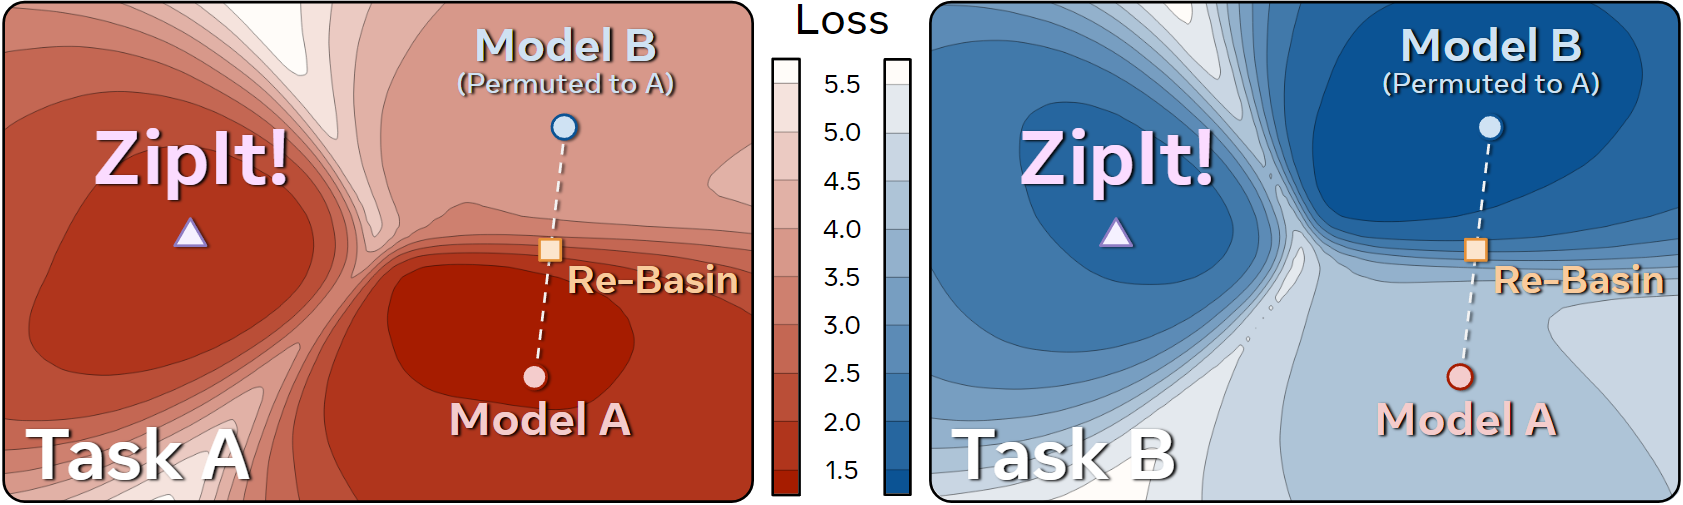
\includegraphics[width=\linewidth]{figures/imgs/loss_landscapes.png}
  % \newline
  % \vspace{-0.5em}
  \caption{{\bf Task Loss Landscapes} for models in Tab.~\ref{tab:cifar50+50}. % Prior work fails on merging models trained on different tasks: 
  \modela{Model A} and \modelb{Model B} lie in low loss basins for their own tasks, but \textit{not for the other task}.
  % While \modelb{Model B} lies in a low loss basin for \modelb{Task B}, it doesn't for \modela{Task A}, even after permuting it to \modela{Model A}.
  % because permuted models for \modela{Task A} likely \textit{do not} lie in a low loss basin for \modelb{Task B}.
  Thus, any interpolation between \modela{Model A} and a permuted \modelb{Model B} (e.g., Git Re-basin) lies outside the minima \textit{for both tasks} and thus performs poorly. In contrast, \name{}\ improves the merge by finding a model that lies in a low loss basin for both.
  % by finding a loss basin common to both tasks.
  % Git Re-Basin~\citet{ainsworth2022git} assumes the two models likely lie in the same loss basin \textit{modulo permutation} and interpolates between them. However, this is substantially less likely when the models are trained on \textit{different} tasks, here shown for disjoint class sets of CIFAR-100. While \modela{A} and \modelb{B} lie in basins on their respective tasks, these \textit{are not} shared across tasks. Thus, Git Re-Basin's interpolation performs \textit{worse} than the original's. In contrast, our method \name{}\ significantly improves the merge by finding a basin common to both tasks. 
  }
  \label{fig:loss_basin}
\end{figure}
\paragraph{Problems with Permutation.}
Eq.~\ref{eq:rebasin} relies on the likelihood of \modelb{model B} lying in the same basin as \modela{model A} after permutation being high. However, this is far less likely when the models are trained on different tasks, as each model optimizes for basins containing distinct task-specific information. In this case the optimal permutation of \modelb{model B} to \modela{model A} still lies in a strong basin on \modelb{task B} but \textit{doesn't} lie in a basin on \modela{task A}, as shown in Figure~\ref{fig:loss_basin}. This causes the interpolated model to perform worse than either the two original models. Thus, we explore alternative merging methods.
% As we show in Figure~\ref{fig:loss_basin}

% While Eq.~\ref{eq:rebasin} works decently well for models trained on the same task, its underlying assumptions break down when the models are trained on \textit{different} tasks. As we show in Fig.~\ref{fig:loss_basin}, these models may not lie in the same loss basin after permutation. In this case, \modelb{Model B}'s optimal permutation lies in a \textit{similar} yet distinct basin to \modela{Model A}. Because the two models are actually in \textit{different basins}, the interpolated result actually has a \textit{lower} accuracy than either of the two original models. This motivates us to explore alternative methods for merging.


% The idea of permutation-based model merging (e.g. Git Re-Basin \cite{ainsworth2022git}) stems from mode connectivity \cite{entezari2021role}, where it has been conjectured that models with different initializations trained on the same data lie in the same \textit{loss basin} (i.e., region of low loss or high accuracy) modulo permutation (as most neural networks can be permuted internally without affecting their outputs). As we show in Fig.~\ref{fig:loss_basin}, this does not hold in our setting where the two models are trained on different tasks. In this case, \modelb{Model B}'s optimal permutation lies in a \textit{similar} yet distinct basin to \modela{Model A}. Because the two models are actually in \textit{different basins}, the interpolated result actually has a \textit{lower} accuracy than either of the two original models. This motivates us to explore alternative methods for merging.

% \subsection{Contributions}
% In addition to extending the problem of model merging to multiple tasks, we further motivate our two primary contributions. 
% Permutation methods focus on exactly mapping every feature in \modela{Model A} to \modelb{Model B} when merging them. 
% This inherently assumes that features across the models are similar, and more likely occurs when the models are trained on the same dataset. 
% However, the likelihood is much smaller when models are trained on different tasks, because their features become less correlated over the course of the network \citep{kornblith2019similarity}. 
% In this case\footnote{unless very rare conditions hold --- please see Appendix~\ref{appendix:postulate2_footnote}}, no permutation may exist to merge the models. 
% Instead, these divergent features between models should be processed via a method other than permutation.

% \paragraph{Merging Within Models.} 
% One way to address this problem is to exploit feature similarity \textit{within} \modela{Model A} and allows these features to be combined with others in \modela{Model A}, while permuting those similar \modelb{Model B} together.
% More specifically, this extends model merging by merging any combination of similar features \textit{within} models, and \textit{across} them.
% Notably, this supports many-1 and many-none in addition to 1-1 merging.
% First, it supports many-to-1 matching because any similar features within \modela{Model A} can be combined together before being permuted to their similar counterpart in \modelb{Model B}, and vice-versa.
% Second, it supports many-to-none matching because the same combined features may instead by matched to any empty feature in \modelb{Model B} obtained when its own features are merged.
% % \name{} demonstrates the efficacy of \name{} through extensive empirical results---improving accuracy by up to \textbf{20\%} over permutation methods---and we further \textit{prove} its approach is \textbf{strictly} better than permutation methods under certain conditions---Appendix~\ref{appendix:postulate}. 

% \paragraph{Partial Merging.} 
% A second way to address this problem is to simply only merge \modela{Model A} and \modelb{Model B} up to layers whose features are non-divergent.
% The intermediate outputs can then be passed into the unmerged layers in \modela{Model A} and \modelb{Model B} to create a multi-head model. 
% While this solution may increase the overall flop count compared to fully merging the models, it can significantly improve performance. 
% % Notably, \name{} outperforms fully merged models by \textbf{over 15\%} while still keeping most layers merged. 




% \paragraph{Permutation Limitations.}
% Models trained on the same task only need to be reasonably sized for permutation based methods to achieve decent performance because they quickly learn redundant features. This is not necessarily true when the models are trained on different tasks, and we consistently find that Eq.~\ref{eq:rebasin} requires \textit{significantly larger} sized models to achieve comparable merging performance (E.g., Figure~\ref{fig:model_size}). However, we find that better merging can be achieved with dramatically lower model size if feature redundancy within models can also be exploited. This is because rather than forcibly merging non-redundant features between models, these can instead be merged with their redundant counterparts in the model. Thus, we make the following conjecture: 
% \begin{center}
%     \textit{Methods that jointly exploit feature redundancy within and across the models are significantly more interpolatable than permutation based approaches, even for dramatically lower model sizes.}
% \end{center}
% The above conjecture is an extension of that from \cite{entezari2021role} and specifies that a lower model size is needed. This is illustrated by Figure~\ref{fig:loss_basin}. We provide both theoretical and empirical evidence in support of this conjecture. Postulate A (Please see Appendix ?) shows its validity in a certain limited setting, driving observations supporting the conjecture found through extensive experimentation.
